\documentclass[a4paper,fleqn]{cas-dc}

\usepackage[authoryear,longnamesfirst]{natbib}
\usepackage{amsmath,amssymb,amsfonts}
\usepackage{booktabs}
\usepackage{multirow}
\usepackage{graphicx}
\usepackage{xcolor}
\usepackage{hyperref}

\newcommand{\method}{Complement Prompting + Score Fusion}
\newcommand{\samthree}{SAM~3}
\newcommand{\samtwo}{SAM~2}
\newcommand{\clip}{CLIP}
\newcommand{\known}{\textit{known}}
\newcommand{\unknown}{\textit{unknown}}

\begin{document}
\let\WriteBookmarks\relax
\renewcommand{\topfraction}{0.95}
\renewcommand{\dbltopfraction}{0.95}
\renewcommand{\bottomfraction}{0.85}
\renewcommand{\textfraction}{0.05}
\renewcommand{\floatpagefraction}{0.75}
\renewcommand{\dblfloatpagefraction}{0.75}
\setcounter{topnumber}{3}
\setcounter{bottomnumber}{2}
\setcounter{totalnumber}{5}
\setcounter{dbltopnumber}{2}

\shorttitle{Complement Prompting for Open-World Dense Segmentation}
\shortauthors{Author et al.}

\title[mode=title]{Complement Prompting for Open-World Dense Segmentation}

\author[1]{Author Name}
\ead{author@example.com}
\affiliation[1]{organization={Affiliation},
  addressline={Address},
  city={City},
  postcode={000000},
  country={Country}}

\begin{abstract}
Open-world dense segmentation systems silently misclassify pixels from unseen classes by forcing them into known categories, creating a high-risk failure mode in safety-critical settings. In prior diagnostic work, we formalized this failure as Structured Abstention Segmentation (SASeg) and identified a key bottleneck in the unseen-unknown setting: anomaly scores can already rank unknown pixels well, but the system fails to generate candidate masks that spatially align with unknown regions. This paper directly closes that open problem. We propose \method, a zero-shot mechanism that leverages concept-promptable foundation models to enumerate known-class masks, extract their foreground complement as unknown candidates, and fuse those candidates with SASeg's ensemble anomaly score at the mask level. The method requires no unknown-class supervision, no modification of the foundation model, and no additional training. Controlled intervention experiments directly confirm the earlier bottleneck diagnosis: stronger scoring alone yields little benefit, stronger candidates yield the dominant improvement, and combining both brings no decisive additional gain. On PASCAL VOC 2012, the proposed method raises A2 Unknown F1 from 0.008 to 0.372 while preserving Known mIoU at 0.746. On RoadAnomaly21 and RoadObstacle21, it improves Unknown F1 from 0.380 to 0.652 and from 0.054 to 0.515, respectively. On dense urban scenes such as Cityscapes, the mechanism yields measurable gains but introduces a known--unknown trade-off; on medical CT benchmarks, it fails because foundation-model concept grounding collapses outside its training modality. A backbone substitution using \samtwo{} and \clip{} partially reproduces the mechanism but remains weaker than native \samthree{} Promptable Concept Segmentation, indicating that the core dependency is a capability combination---class-agnostic mask generation plus concept-level grounding---rather than a specific model instance. These results characterize when concept-promptable foundation models can serve as zero-shot candidate generators for open-world dense segmentation, and explicitly delineate the regimes in which this mechanism succeeds, partially succeeds, and fails.
\end{abstract}

\begin{highlights}
\item We close the candidate-generation open problem identified by SASeg using a zero-shot complement-prompting mechanism.
\item Controlled interventions show that candidate generation, not stronger scoring, is the dominant bottleneck in A2 unseen-unknown structuring.
\item Experiments across six datasets map the effective, trade-off, and failure regimes of concept-promptable foundation models.
\end{highlights}

\begin{keywords}
open-world dense segmentation \sep zero-shot segmentation \sep anomaly segmentation \sep foundation models \sep promptable concept segmentation
\end{keywords}

\maketitle

\section{Introduction}
\label{sec:intro}

\subsection{Open-World Failure in Dense Segmentation}
\label{sec:intro:problem}

Dense segmentation systems are usually trained under a closed-set assumption: every pixel must be assigned to one of the categories observed during training. In deployment, however, scenes inevitably contain unseen objects, structures, or anomalies. Under the closed-set assumption, those pixels are silently forced into the nearest known class, producing predictions that are spatially precise and highly confident, yet semantically wrong. This failure mode is especially concerning in safety-critical settings such as medical imaging, autonomous driving, and industrial inspection, where unfamiliar content may be exactly what downstream users most need to notice.

This problem is not fully captured by the standard framing of unknown handling as confidence thresholding. In dense prediction, the practical requirement is not only to rank unfamiliar pixels as risky, but also to organize them into coherent regions that can support inspection, abstention, or handoff. A scattered uncertainty map is often insufficient for these workflows. What is needed instead is a structured output that explicitly marks the unexplained part of the scene while preserving the segmentation quality of known classes.

Our starting point is therefore a broader view of open-world segmentation: the central challenge is not merely whether unknown content can be detected, but whether it can be represented as a usable dense output under realistic test-time conditions.

% TODO: Add supporting citations for open-world recognition, dense segmentation, and safety-critical deployment.

\subsection{Self-Contained Restatement of the Prior Diagnosis}
\label{sec:intro:prior}

Our prior arXiv preprint introduced Structured Abstention Segmentation (SASeg) and the A1/A2 evaluation protocol to separate seen-unknown structuring from unseen-unknown detection generalization. That work identified a diagnostic gap that is central to the present paper. In the A2 setting, ensemble anomaly signals already achieve strong pixel-level ranking quality, with AUROC often above 0.95 across both medical and natural-image datasets. Yet structured unknown outputs remain essentially unusable: Unknown F1 stays near zero and the union of candidate regions scarcely overlaps the true unknown regions at all. The central implication is that the failure is not primarily a scoring failure. It is a candidate-generation failure.

This paper is written to stand on its own even if the reader does not treat the preprint as an accepted premise. We therefore restate the protocol and the diagnostic problem inside the paper and provide new controlled intervention evidence that independently supports the same conclusion. In this sense, the paper is not merely an incremental extension of SASeg, but a direct attempt to close the specific open problem that SASeg left unresolved: how to generate unknown candidates in the unseen-unknown setting without unknown supervision.

\subsection{Opportunity from Concept-Promptable Foundation Models}
\label{sec:intro:opportunity}

\samthree{} introduces Promptable Concept Segmentation, which accepts noun-phrase prompts and returns masks for matching image regions. This capability changes the design space in an important way. For the first time, a single foundation model provides both concept-level grounding and class-agnostic mask generation closely enough to make test-time unknown candidate generation plausible.

This suggests a simple but previously unavailable route: enumerate the known classes, construct their union as a known explanation of the scene, and treat the remaining foreground complement as a source of unknown candidates. If this works, then the paper's open problem can be attacked entirely at inference time, without modifying the segmentation backbone, retraining the foundation model, or introducing any unknown-class annotations. The key question is whether such a mechanism can actually produce spatially aligned candidates rather than merely another ranking heuristic.

\subsection{Main Findings}
\label{sec:intro:findings}

Our experiments lead to four main findings. First, direct negation-style prompting does not work; the only reliable mechanism is enumeration-then-complement. Second, complement candidates have extremely high recall but require score fusion to avoid severe degradation of known-class segmentation. Third, controlled interventions confirm that stronger candidates, not stronger scores, drive the main A2 gain. Fourth, the mechanism is strongly conditioned by two factors: concept-grounding coverage and scene density. Together these factors produce three empirical regimes across datasets: effective, partial with trade-off, and outright failure.

These findings matter for more than one particular model. They show that the candidate-generation bottleneck can be closed in some regimes by a concept-promptable foundation model, but they also show exactly where the mechanism breaks: dense scenes with incomplete grounding coverage and modalities that lie outside the foundation model's visual grounding domain.

\subsection{Contributions}
\label{sec:intro:contrib}

This paper makes the following contributions:
\begin{enumerate}
  \item We propose \method, a zero-shot unknown candidate generation mechanism that closes the candidate-generation open problem identified in SASeg without extra training, unknown supervision, or foundation-model modification.
  \item We provide controlled intervention evidence showing that candidate generation is the dominant bottleneck in A2 unseen-unknown structuring, while stronger scoring alone is insufficient.
  \item We characterize the method's applicability boundary across six datasets, identifying effective, trade-off, and failure regimes and relating them to concept-grounding coverage and scene density.
  \item We show that the mechanism depends on a capability combination---class-agnostic mask generation plus concept-level grounding---rather than on \samthree{} as a single specific model.
\end{enumerate}

Taken together, the paper's contribution is therefore not simply a better result on one benchmark. Rather, it closes a previously diagnosed open problem, validates the nature of that problem with intervention-style evidence, and maps the conditions under which the proposed solution succeeds or fails.

\section{Related Work}
\label{sec:related}

\subsection{Prior Diagnostic Work: SASeg}
\label{sec:related:saseg}

This paper directly extends the diagnostic thread initiated by SASeg, a prior arXiv preprint by the same authors. SASeg introduced the Structured Abstention Segmentation formulation and the A1/A2 protocol, and it identified the key empirical phenomenon that motivates the present work: in the unseen-unknown setting, dense segmentation models can exhibit strong pixel-level anomaly ranking while still failing almost completely at structured unknown prediction. The present paper should therefore be read neither as a separate problem formulation nor as a conventional successor method paper, but as a direct attempt to close the specific open problem that SASeg left unresolved.

At the same time, SASeg is not treated here as an unquestionable premise. Because it remains a preprint rather than a peer-reviewed canonical benchmark, this paper restates its setup in self-contained form and supplies new intervention-style evidence for the same bottleneck diagnosis. The distinction matters. The contribution of the present work is not only that it inherits SASeg's framing, but that it converts the earlier correlational observation into a direct test of what actually improves A2 structured unknown quality.

% TODO: Cite the SASeg preprint explicitly as a preprint and state that A1/A2 is inherited but restated self-containedly.

\subsection{Open-Set Recognition and OoD Detection}
\label{sec:related:osr}

Open-set recognition and out-of-distribution detection provide the conceptual starting point for unknown handling, but they typically operate at a different output granularity from the one studied here. Classical open-set recognition methods focus on rejecting unseen classes at the image or sample level by calibrating confidence, modeling open-space risk, or explicitly reserving representation space for unknowns. Later OoD detection work similarly concentrates on ranking whether an input belongs to the training distribution, often through maximum-softmax baselines, energy-based scores, virtual outlier synthesis, or other confidence-oriented criteria.

These lines of work are highly relevant because they supply the scoring language that underlies much of modern unknown detection. However, they do not by themselves solve the dense-structuring problem. A pixel-level score or a sample-level rejection signal does not tell the system how to assemble coherent unknown regions inside a segmentation output. The core distinction emphasized in this paper is therefore not between one score and another, but between \emph{ranking} and \emph{structuring}. Our intervention results are best understood as a direct continuation of this distinction: strong scores are useful, but only after spatially aligned candidates have been generated.

This places the paper adjacent to, but not inside, the standard OSR/OoD literature. We inherit the concern with unseen-category uncertainty, yet our main question is different: what is required to transform unknown evidence into a region-level abstention output that can coexist with high-quality known-class segmentation?

% TODO: Add citations for OpenMax, ARPL, placeholder learning, MSP, energy-based OoD, virtual outlier synthesis, and a survey that covers dense OoD detection.

\subsection{Anomaly Segmentation on Road Scenes}
\label{sec:related:anomaly}

Road-scene anomaly segmentation is the closest task-specialized literature to the practical motivation of this paper, especially through the Segment Me If You Can (SMIYC) benchmark family and related methods. That literature is designed around detecting unusual obstacles or anomalies in driving scenes under zero or limited anomaly supervision, often using task-specific architectures, auxiliary outlier exposure, synthetic anomaly generation, or dedicated post-processing pipelines. It is therefore more directly optimized for anomaly segmentation as a benchmark task than the method proposed here.

The relation between that literature and the present paper is subtle. On the one hand, SMIYC-style methods are an important external check because they provide an established evaluator and a distinct notion of success at both pixel and instance levels. On the other hand, they are not the primary target of our claims. Our method is not trained end-to-end for road-scene anomaly segmentation, and we do not present the SMIYC results as leaderboard competition. Instead, those results serve as cross-benchmark mechanism validation: they test whether a candidate-generation mechanism originally designed to address SASeg's A2 bottleneck still produces directionally consistent gains under an independent benchmark protocol.

This difference in task framing is important for interpretation. The central contribution of this paper is not a new anomaly-segmentation benchmark winner, but a mechanism-level account of how zero-shot candidate generation can improve structured unknown output. The SMIYC results are valuable precisely because they expose both the transferability of that mechanism and its limitations, particularly the tension between pixel-level purity and instance-level completeness.

% TODO: Add citations for SMIYC, representative anomaly-segmentation methods such as outlier-aware segmentation / Mask2Anomaly / RbA, and the official benchmark/evaluator papers.

\subsection{Query-Based Segmentation and Foundation Models}
\label{sec:related:foundation}

Query-based segmentation architectures are relevant because they established mask-level prediction as a natural interface for dense visual output. Rather than treating segmentation as independent per-pixel classification, models in the MaskFormer, Mask2Former, Mask DINO, and related families treat dense prediction as a set-prediction or mask-parsing problem. This conceptual move matters here because our method also reasons in terms of candidate masks rather than only per-pixel scores. In that sense, the paper aligns more naturally with region-level parsing than with classical confidence-threshold segmentation.

The foundation-model side of the story adds a second ingredient. The SAM family progressively expanded promptability from geometric interaction to broader segmentation use cases, and the emergence of concept-promptable segmentation changes what can be done at inference time. The present paper relies specifically on the ability to recall known concepts as masks and then treat the residual foreground as a source of unknown candidates. This is not how prior query-based segmentation papers frame the problem, nor is it how most earlier SAM-based applications use the model.

The main distinction, then, is not that prior segmentation architectures lacked masks, but that they did not provide a direct route from concept grounding to zero-shot unknown candidate generation. Our method uses a concept-promptable foundation model not as a complete segmentation solution, but as a structured proposal mechanism layered on top of a frozen open-world segmentation system.

% TODO: Add citations for MaskFormer / Mask2Former / Mask DINO and for the relevant SAM-family papers, especially the concept-promptable variant used here.

\subsection{Foundation-Model Adaptation}
\label{sec:related:adapt}

Another relevant line of work adapts large segmentation foundation models to new domains through fine-tuning, lightweight adapters, LoRA-style parameter-efficient updates, or domain-specialized retraining. Medical variants of SAM are especially relevant because they demonstrate that strong geometric or promptable segmentation performance in one domain does not automatically transfer to another. These works pursue better domain fit by modifying the model.

This paper takes a deliberately different route. We do not adapt the foundation model to any target domain. Instead, we ask a narrower but more diagnostic question: when is the \emph{native} zero-shot capability of a concept-promptable model already sufficient to serve as an unknown candidate generator, and what happens when that capability is absent? This is why the medical CT results are so important. They show not merely that performance drops out of domain, but that the entire complement mechanism fails once known-concept grounding collapses.

Relative to adaptation work, the contribution of this paper is therefore not improved transfer through additional training. It is a capability-boundary characterization. The method works when the foundation model can explain enough of the known scene to make the residual meaningful, and it fails when that prerequisite is violated. Future domain-adapted concept-promptable models may remove some of the current failure cases, but they would do so by strengthening the capability combination identified here rather than by changing the logic of the pipeline itself.

% TODO: Add citations for MedSAM, SAM-HQ, LoRA-style SAM adaptation, and related domain-adaptation work for promptable segmentation models.

\section{Problem Setup}
\label{sec:problem}

\subsection{Structured Abstention Segmentation and the A1/A2 Protocol}
\label{sec:problem:a1a2}

We adopt the Structured Abstention Segmentation perspective introduced in SASeg, but restate it here in a self-contained form. Let the training label space be divided into two parts: a set of known classes $\mathcal{K}$ that are meant to be segmented explicitly, and a set of regions that should not be forced into $\mathcal{K}$. At test time, the system must output a dense prediction that preserves the structure of known classes while also marking pixels belonging to out-of-scope content as \unknown{} rather than misclassifying them as known.

The A1/A2 protocol separates two related but distinct capabilities. In A1, unknown regions are drawn from categories that are available as unknown during development, so the task primarily tests whether the model can organize an \unknown{} output channel into coherent masks. In A2, the model is evaluated on previously unseen unknown categories at test time. This second setting is much more demanding: the model must generalize beyond the specific unknown patterns available during development and produce structured \unknown{} outputs for content it has never encountered as unknown before.

Formally, let $\mathcal{U}_{\text{seen}}$ denote the set of unknown categories available during development and let $\mathcal{U}_{\text{unseen}}$ denote unknown categories that appear only at test time. A1 evaluates structured abstention on $\mathcal{U}_{\text{seen}}$, whereas A2 evaluates structured abstention on $\mathcal{U}_{\text{unseen}}$. The main focus of this paper is A2, because that is where the diagnostic gap between pixel-level ranking and structured output is most pronounced and where the candidate-generation problem becomes the dominant bottleneck.

This distinction is important for interpreting the proposed method. \method{} is not intended to improve a model's semantic understanding of unknown categories through training. Instead, it augments inference by supplying spatial candidates that a frozen anomaly-scoring pathway can evaluate. Its success or failure should therefore be read specifically through the lens of A2 unseen-unknown structuring.

\subsection{Evaluation Metrics}
\label{sec:problem:metrics}

The primary evaluation reports both known-side and unknown-side quality because a useful open-world segmentation system must satisfy both constraints at once:
\begin{itemize}
  \item Known mIoU for the segmentation quality of known classes.
  \item Unknown F1, IoU, precision, and recall for structured unknown outputs.
  \item AUROC, AUPR, and FPR@95 for pixel-level ranking quality where appropriate.
\end{itemize}

Known mIoU measures whether the system preserves its ability to parse the classes it is actually supposed to segment. Unknown F1 and IoU measure whether the system can output a coherent \unknown{} region rather than a scattered confidence field. Unknown precision and recall are especially important in this paper because the proposed mechanism deliberately moves along a candidate-purity versus candidate-coverage trade-off. Finally, AUROC, AUPR, and FPR@95 characterize the quality of pixel-level anomaly ranking independently of whether those pixel scores can be assembled into useful masks.

The central methodological point of the paper is that these two levels of evaluation must not be conflated. High AUROC may coexist with near-zero Unknown F1, which means that a model can know something is wrong at the pixel level without being able to produce a structured abstention output. Much of the paper's argument is built on precisely this separation.

\subsection{What Counts as Solving the A2 Bottleneck}
\label{sec:problem:bottleneck}

Under this formulation, solving the A2 bottleneck does not simply mean improving a scalar anomaly score. It means increasing structured unknown quality while preserving known-class segmentation quality. A method that raises unknown recall by flooding the image with false \unknown{} regions is not sufficient, just as a method that preserves known mIoU by predicting almost no \unknown{} pixels is not sufficient. The problem is inherently joint.

This framing also clarifies why our comparison logic is organized around interventions rather than only around end metrics. If stronger scoring alone cannot improve Unknown F1, whereas stronger candidates can, then the missing capability is structural rather than statistical. This is the core claim that \method{} is designed to test.

\section{Method}
\label{sec:method}

\subsection{Overview}
\label{sec:method:overview}

Our goal is to improve A2 unseen-unknown structuring without retraining the segmentation model and without introducing unknown-class supervision. We therefore treat SASeg as a fixed source of pixel-level anomaly evidence and add a separate inference-time candidate-generation path built on top of a concept-promptable foundation model. The resulting pipeline has three stages: known-class enumeration, complement-based candidate generation, and mask-level score fusion.

At a high level, the method works as follows. We first query the foundation model with the vocabulary of known semantic classes and union the returned masks into an estimate of the image foreground already explained by known concepts. We then take the foreground complement of that union and use a class-agnostic mask generator to partition the remaining regions into candidate unknown masks. Finally, we score each candidate with the frozen SASeg anomaly signal and keep only masks whose aggregated score exceeds a validation-selected threshold. This design deliberately separates two functions that the experiments later show should not be conflated: candidate generation provides structure, while score fusion provides selectivity.

The method is intentionally simple in order to test a specific hypothesis. If the main A2 bottleneck is indeed the absence of spatially aligned candidates rather than weak anomaly scores, then supplying strong zero-shot candidates should produce the dominant gain even when the underlying scoring model remains unchanged. The controlled intervention results in Section~\ref{sec:exp:intervention} are designed around this prediction.

% TODO: Insert pipeline figure.
\begin{figure*}[!t]
  \centering
  \fbox{\rule{0pt}{2.1in}\rule{0.95\textwidth}{0pt}}
  \caption{Pipeline overview placeholder. Replace with a schematic showing known-class prompting with \samthree{}, known-union construction, foreground complement extraction, class-agnostic candidate generation, and mask-level score fusion with SASeg.}
  \label{fig:pipeline}
\end{figure*}

\subsection{Complement Prompting}
\label{sec:method:complement}

Let $I$ denote an input image and let $\mathcal{V}_{\text{known}} = \{c_1, \dots, c_K\}$ be the known-class vocabulary inherited from the SASeg protocol. For each known class $c_k$, we query \samthree{} Promptable Concept Segmentation to obtain a set of masks corresponding to image regions grounded to that concept. We denote the union of all returned known masks by
\begin{equation}
M_{\text{known}} = \bigcup_{k=1}^{K} M_k.
\end{equation}
The goal of this stage is not to produce the final segmentation, but to estimate which parts of the image can already be explained by known concepts.

We then define a foreground complement region
\begin{equation}
M_{\text{comp}} = M_{\text{fg}} \setminus M_{\text{known}},
\end{equation}
where $M_{\text{fg}}$ denotes the image foreground region used by the pipeline. Intuitively, $M_{\text{comp}}$ contains everything in the scene that is not currently covered by the known-class explanation. If the foundation model grounds the known concepts well, then unknown objects should survive inside this complement with high recall, even though the complement may also contain leaked known pixels.

Within $M_{\text{comp}}$, we invoke a class-agnostic mask generator to enumerate a candidate set $\{C_i\}_{i=1}^{N}$. This step converts a coarse foreground complement into discrete region proposals that can be filtered and scored downstream. We apply two lightweight geometric filters before score fusion:
\begin{equation}
\text{area}(C_i) > \tau_{\text{area}},
\end{equation}
and
\begin{equation}
\text{overlap}(C_i, M_{\text{known}}) < \tau_{\text{overlap}},
\end{equation}
where the overlap term suppresses proposals that remain dominated by already explained known content.

The specific form of this stage follows directly from the empirical constraints of the prompting interface. We tested direct negation prompts, generic anomaly-style prompts, and negative-exemplar variants, but these alternatives failed to return usable unknown masks. The only prompt form that consistently produced meaningful candidate regions was enumeration-then-complement. For this reason, complement prompting should be understood not as an arbitrary prompt-engineering choice, but as the only viable operationalization of unknown candidate generation under the current concept-promptable interface.

\subsection{Score Fusion}
\label{sec:method:fusion}

Complement prompting yields high-recall candidates, but using all such candidates directly leads to severe known-class degradation because leaked known regions are also included. We therefore fuse each candidate with the frozen SASeg anomaly signal. Let $p_{\text{best}}(x)$ denote the highest known-class confidence at pixel $x$ under SASeg, and let $U_{\text{union}}(x)$ denote the auxiliary uncertainty term inherited from the SASeg A2 inference path. For each candidate mask $C_i$, we compute its aggregated score as
\begin{equation}
s_i = \frac{1}{|C_i|} \sum_{x \in C_i} \left[0.8 \cdot \left(1 - p_{\text{best}}(x)\right) + 0.2 \cdot U_{\text{union}}(x)\right].
\label{eq:fusion}
\end{equation}
Only candidates whose score exceeds a threshold $\tau_{\text{fusion}}$ are retained as final unknown outputs:
\begin{equation}
\hat{Y}_{\text{unk}} = \bigcup_{i: s_i > \tau_{\text{fusion}}} C_i.
\end{equation}

This aggregation step is crucial because it converts SASeg's already strong pixel-level ranking ability into a region-level selection signal. In other words, the score pathway is not asked to invent the unknown structure by itself; it only decides which already proposed masks should survive.

We use the terms \textbf{L1} and \textbf{L2} to distinguish two versions of the method throughout the experiments. L1 refers to using the complement-derived candidate set directly, without score-based filtering. Operationally, this corresponds to setting the fusion threshold to zero and accepting every surviving candidate after the geometric filters. L2 refers to the full method, in which the candidates are further filtered by the mean mask score in Eq.~\eqref{eq:fusion}. This distinction is important for interpretation: L1 is not a competing baseline, but an ablation that isolates the effect of candidate generation before score fusion.

\subsection{Why Both Components Are Needed}
\label{sec:method:design}

The design of the method follows the central diagnosis of the paper: the A2 failure is a mismatch between strong ranking signals and weak spatial candidates. Complement prompting and score fusion therefore address different parts of the failure.

Complement prompting addresses the structural side. By enumerating known concepts and taking their complement, it supplies candidate regions that are spatially aligned with unknown content and typically achieve near-saturated recall in the positive natural-image settings. However, this step alone is too permissive. Because concept grounding is not perfect, the complement often contains leaked known regions, especially in dense scenes. This is why the raw-candidate L1 variant can produce very high unknown recall while simultaneously destroying Known mIoU.

Score fusion addresses the selection side. SASeg already provides high-quality pixel-level ranking signals in A2, but those signals are not sufficient on their own to assemble coherent unknown masks. Once complement prompting supplies spatial candidates, the same scoring information becomes highly useful as a mask-level filter. In this sense, the two components are complementary rather than redundant: candidate generation supplies the structure that scoring lacks, and scoring supplies the purification that raw complement masks lack.

This division of labor leads to two falsifiable expectations that are tested later in the paper. First, strengthening scores without changing candidates should have little effect on structured unknown quality. Second, strengthening candidates while keeping the original score pathway should produce the dominant gain. The intervention results in Section~\ref{sec:exp:intervention} match exactly this pattern.

\subsection{Prompt-Form Alternatives and Threshold Selection}
\label{sec:method:threshold}

We compare four prompt forms in the ablation study: direct negation, generic concept prompts, enumeration-then-complement, and negative exemplars. The empirical result is unambiguous: only enumeration-then-complement produces usable unknown candidates. Direct negation and generic prompts fail because the current interface does not ground them into coherent unknown regions, while negative-exemplar prompting remains ineffective even after engineering additional prompt templates. This outcome motivates the final method design reported in this section.

The three thresholds $\tau_{\text{area}}$, $\tau_{\text{overlap}}$, and $\tau_{\text{fusion}}$ are selected on validation data and then frozen before the main evaluation. Their role is intentionally modest on easy scenes and more substantive on dense scenes. On VOC, the method is largely insensitive to threshold choice, which indicates that candidate quality is already strong and filtering only performs light cleanup. On Cityscapes, threshold choice matters much more because complement regions contain substantially more known leakage, making candidate filtering part of the mechanism rather than a minor post-processing detail.

In the main experiments, the best validation settings are dataset-specific. VOC uses $\tau_{\text{area}} = 128$, $\tau_{\text{overlap}} = 0.5$, and $\tau_{\text{fusion}} = 0.5$, while Cityscapes uses $\tau_{\text{area}} = 64$, $\tau_{\text{overlap}} = 0.8$, and $\tau_{\text{fusion}} = 0.1$. We report these values explicitly because they help interpret the later trade-off analysis: the looser fusion threshold on Cityscapes is not an arbitrary tuning artifact, but an attempt to preserve unknown recall in a regime where concept grounding is visibly less complete.

\section{Experiments}
\label{sec:exp}

\subsection{Experimental Setup}
\label{sec:exp:setup}

\subsubsection{Dataset Roles}
\label{sec:exp:roles}

Table~\ref{tab:dataset-roles} defines the narrative role of each dataset in the paper. This table is important because it prevents the road-scene benchmarks from being misread as a pure leaderboard-comparison section and frames the medical experiments as deliberate boundary analysis rather than as hidden negative results.

\begin{table*}[!t]
  \caption{Role of each dataset in the paper's experimental narrative.}
  \label{tab:dataset-roles}
  \centering
  \begin{tabular}{llll}
    \toprule
    Dataset & Data type & Narrative role & Primary evaluation \\
    \midrule
    PASCAL VOC 2012 & Natural images, object-isolated & Primary positive result & Full-system A2 \\
    Cityscapes & Natural images, dense urban scenes & Boundary / trade-off case & Full-system A2 \\
    RoadAnomaly21 & Road-scene anomalies & Cross-benchmark positive & Unified + SMIYC official \\
    RoadObstacle21 & Road-scene obstacles & Cross-benchmark positive & Unified + SMIYC official \\
    Synapse & Abdominal CT & Failure boundary & Qualitative + candidate quality \\
    AMOS22 & Abdominal CT & Failure boundary & Qualitative + candidate quality \\
    \bottomrule
  \end{tabular}
\end{table*}

\subsubsection{Checkpoints, Protocol, and Implementation Notes}
\label{sec:exp:impl}

The main positive-domain experiments use the SASeg A2 checkpoints trained on VOC and Cityscapes, respectively. For the road-scene extension experiments, we deliberately reuse the Cityscapes A2 checkpoint on both RoadAnomaly21 and RoadObstacle21 without additional training. This cross-dataset setting helps isolate the contribution of the inference-time candidate mechanism from any gain that might arise from training directly on road-anomaly data.

Unless otherwise noted, the main evaluation follows the unified SASeg protocol and reports both known-side and unknown-side quality. The foundation-model branch is kept frozen throughout. All prompt vocabularies are constructed from the dataset's known-class names, and the complement pathway is evaluated only at inference time. Thresholds for the underlying SASeg score path are selected on validation data in the usual way, and the complement-specific thresholds are tuned on validation data and then frozen before the reported experiments.

For VOC, the full-system evaluation uses the SASeg checkpoint \texttt{voc2012\_a2/best.pth} and evaluates on 1,449 validation images. For Cityscapes, we use \texttt{cityscapes\_a2/best.pth} on 500 validation images. For the official SMIYC public-validation runs, we retain the Cityscapes checkpoint and run the benchmark evaluator unchanged. This separation between training protocol and evaluation protocol is important to our claim: the paper is not proposing a new task-specialized anomaly segmenter, but an inference-time mechanism that can be attached to a pre-existing open-world dense segmentation model.

\subsection{Main Results: Full-System A2 Evaluation}
\label{sec:exp:main}

% TODO: Replace the placeholder table body with final numbers from full_system_eval and stage29.
\begin{table*}[!t]
  \caption{Full-system A2 evaluation under the unified SASeg protocol.}
  \label{tab:main-results}
  \centering
  \begin{tabular}{llllllll}
    \toprule
    Dataset & Method & Known mIoU & Unknown F1 & Unknown IoU & Unknown Precision & Unknown Recall & AUROC$_{\text{fg}}$ \\
    \midrule
    VOC & Baseline (SASeg A2) & 0.746 & 0.008 & 0.004 & 0.005 & 0.012 & 0.980 \\
    VOC & L1 & 0.334 & 0.175 & 0.096 & 0.096 & 0.994 & 0.731 \\
    VOC & L2 & 0.746 & 0.372 & 0.228 & 0.231 & 0.954 & 0.981 \\
    Cityscapes & Baseline (SASeg A2) & 0.624 & 0.017 & 0.008 & 0.011 & 0.032 & 0.963 \\
    Cityscapes & L1 & 0.279 & 0.035 & 0.018 & 0.018 & 0.987 & 0.781 \\
    Cityscapes & L2 & 0.583 & 0.074 & 0.038 & 0.047 & 0.140 & 0.962 \\
    RA21 & Baseline & --- & 0.380 & 0.234 & 0.433 & 0.338 & 0.828 \\
    RA21 & L2 & --- & 0.652 & 0.484 & 0.506 & 0.916 & 0.885 \\
    RO21 & Baseline & --- & 0.054 & 0.028 & 0.037 & 0.103 & 0.949 \\
    RO21 & L2 & --- & 0.515 & 0.347 & 0.423 & 0.659 & 0.960 \\
    \bottomrule
  \end{tabular}
\end{table*}

The VOC result is the paper's strongest primary positive case: \method{} improves Unknown F1 by roughly 46$\times$ while preserving Known mIoU. Cityscapes shows that the mechanism still helps in dense urban scenes, but only under a clear known--unknown trade-off. The road-scene datasets confirm that the mechanism produces directionally consistent gains even under an external anomaly-segmentation evaluation context.

More specifically, VOC is the clearest success case. The baseline Unknown F1 is only 0.0075 even though AUROC is already 0.9795, reproducing the classic detection--structuring gap. L2 raises Unknown F1 to 0.3719 and Unknown IoU to 0.2284 while Known mIoU changes by only $-0.0003$. The contrast between L1 and L2 is also instructive: raw complement candidates already recover unknown structure with recall 0.9942, but they destroy known-class quality, reducing Known mIoU from 0.7459 to 0.3341. Score fusion is therefore not a minor refinement; it is the component that turns high-recall complement masks into usable structured outputs.

Cityscapes presents a different regime. The baseline again has strong ranking quality (AUROC 0.9627) but poor structured unknown output (F1 0.0167). With the complement pathway and best filter, Unknown F1 rises to approximately 0.074, but Known mIoU drops from 0.6242 to about 0.583. This is a real gain, but not a free one. The dense-scene setting contains substantially more known leakage inside the complement region, so the method improves unknown structuring only by accepting a measurable known-side trade-off. We therefore report Cityscapes as a boundary case rather than as a second clean positive result.

The road-scene datasets provide cross-benchmark confirmation that the mechanism is not specific to the datasets used to develop SASeg. On RoadAnomaly21, L2 improves Unknown F1 from 0.3797 to 0.6520. On RoadObstacle21, where the baseline is particularly weak, L2 improves Unknown F1 from 0.0540 to 0.5148. These results are especially useful because they are obtained by reusing the Cityscapes checkpoint for inference, which weakens the concern that the effect is merely a consequence of dataset-specific training alignment.

\begin{figure*}[!t]
  \centering
  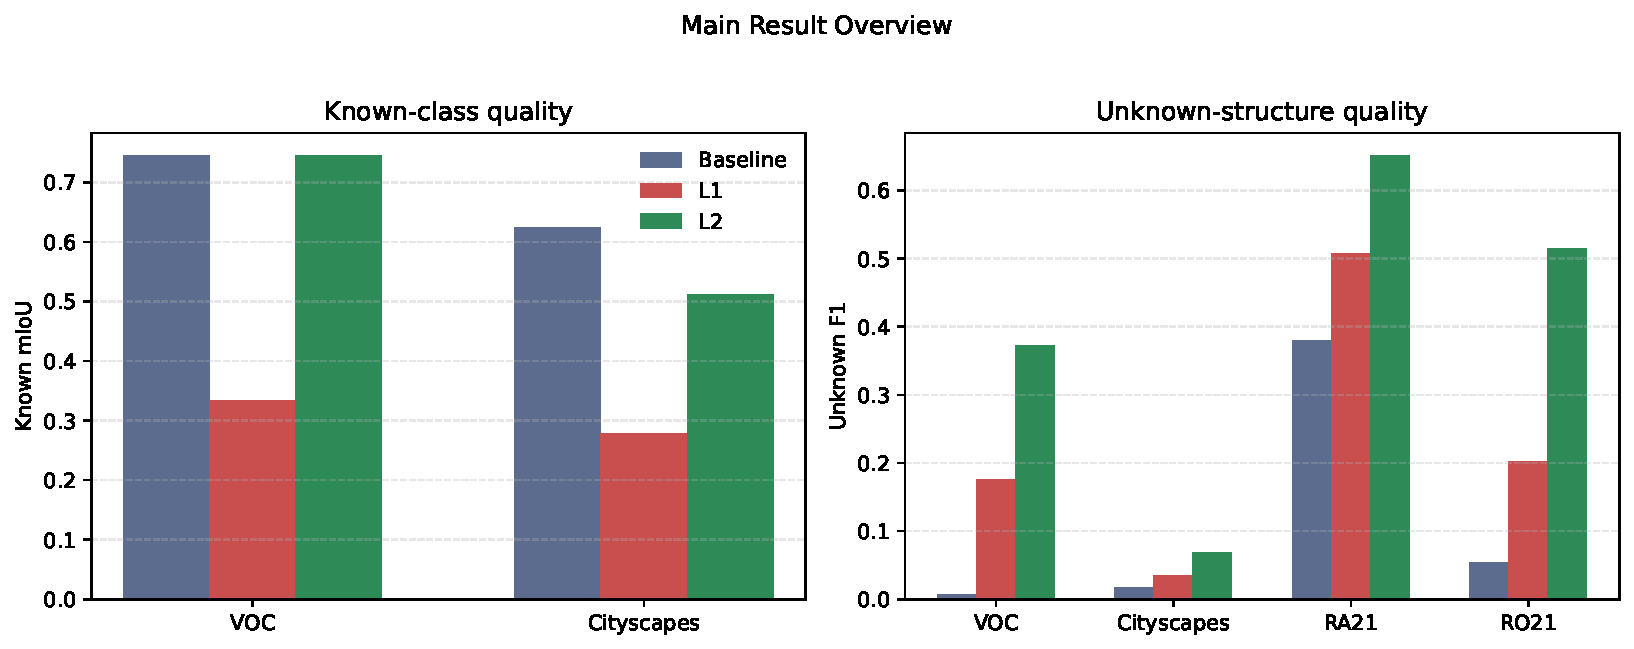
\includegraphics[width=\textwidth]{fig/main_results_overview.pdf}
  \caption{Quantitative overview of the main results. Left: known-class quality on VOC and Cityscapes under Baseline, L1, and L2. Right: unknown-structure quality across VOC, Cityscapes, RoadAnomaly21, and RoadObstacle21. The pattern highlights the central role of score fusion in preserving known performance and the strong positive effect of complement-based candidates on unknown F1.}
  \label{fig:main-results-overview}
\end{figure*}

\begin{figure*}[!t]
  \centering
  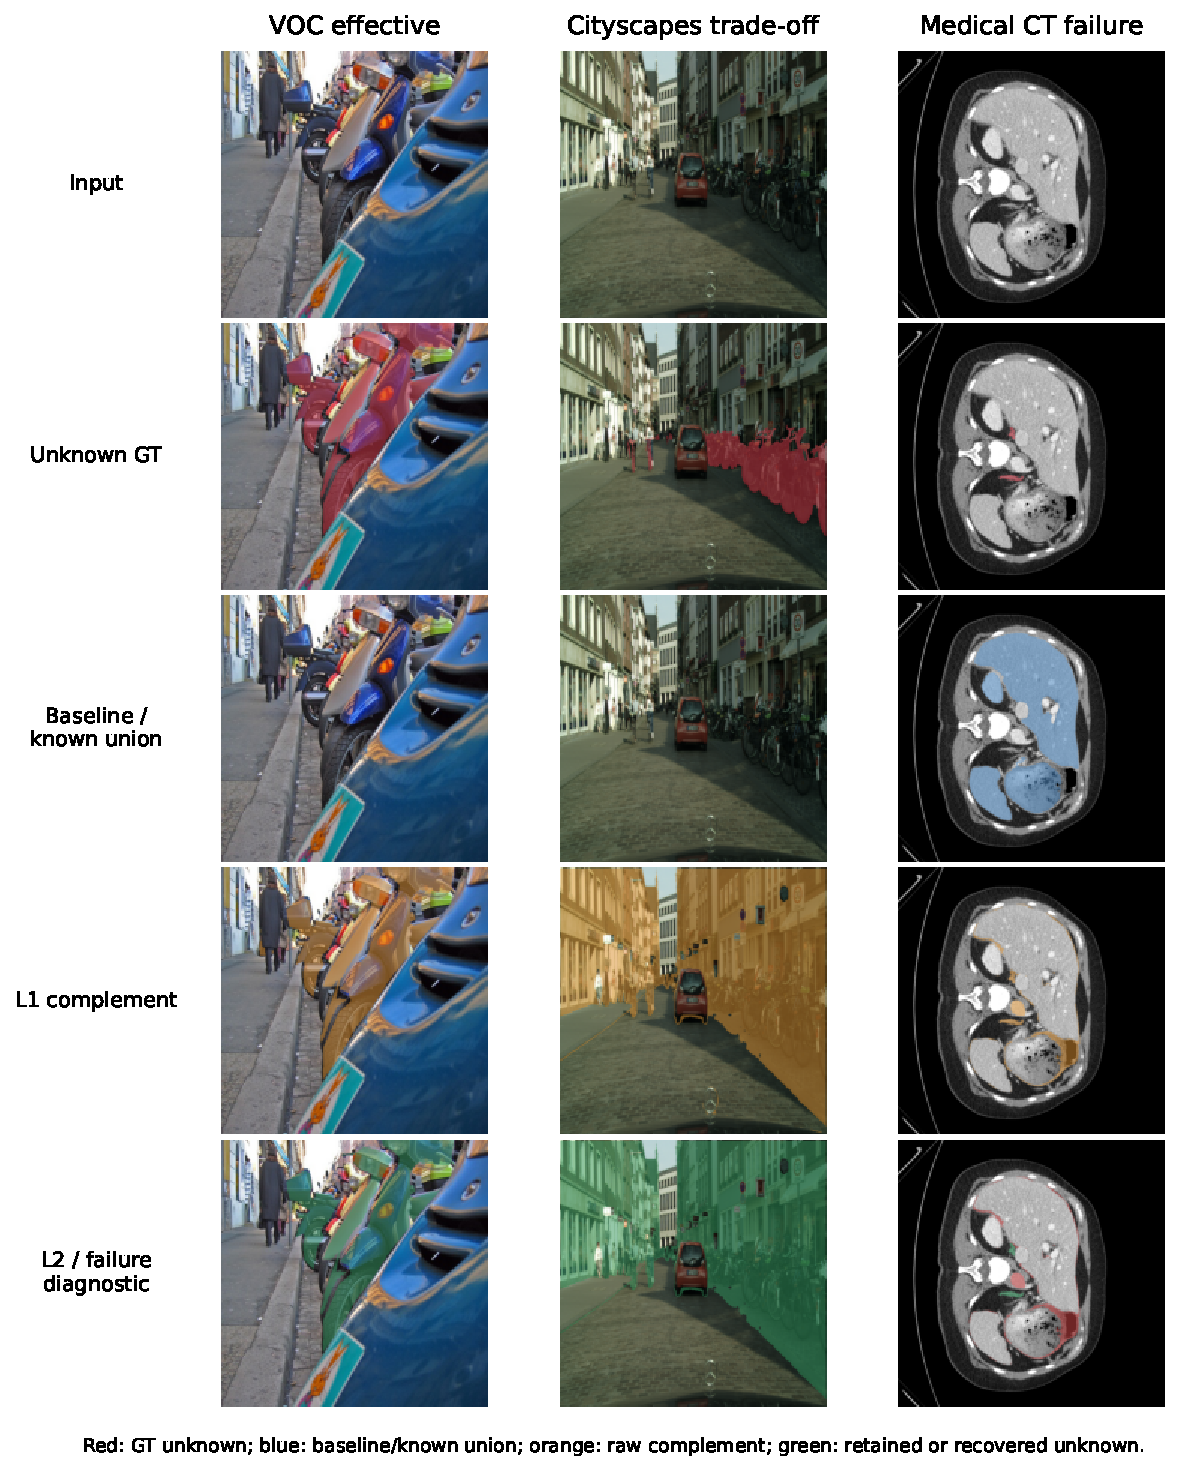
\includegraphics[width=\textwidth,height=0.78\textheight,keepaspectratio]{fig/qualitative_triptych.pdf}
  \caption{Qualitative examples across the three regimes studied in the paper. VOC illustrates the effective regime, where complement candidates recover the unknown object and score fusion preserves known-class quality. Cityscapes illustrates the trade-off regime, where complement prompting improves unknown structure but also admits substantial known leakage in dense scenes. Medical CT illustrates the failure regime, where weak concept grounding prevents the complement from becoming a meaningful unknown-candidate source.}
  \label{fig:qualitative-triptych}
\end{figure*}

\subsection{Controlled Intervention: Candidate Generation vs. Stronger Scoring}
\label{sec:exp:intervention}

This section is the main analysis contribution of the paper. We compare three interventions: A, stronger scoring with fixed candidates; B, stronger candidates with fixed scoring; and A+B, both changes together. The goal is not merely to report a better number, but to determine which component actually addresses the structural bottleneck.

% TODO: Replace with final table layout and add Cityscapes numbers from stage24/stage25.
\begin{table}[!htbp]
  \caption{Controlled intervention results.}
  \label{tab:intervention}
  \centering
  \begin{tabular}{llll}
    \toprule
    Dataset & Setting & Known mIoU & Unknown F1 \\
    \midrule
    VOC & Baseline & 0.746 & 0.008 \\
    VOC & A: stronger score only & 0.745 & 0.007 \\
    VOC & B: stronger candidates only & 0.746 & 0.372 \\
    VOC & A+B: both & 0.745 & 0.377 \\
    Cityscapes & Baseline & 0.624 & 0.017 \\
    Cityscapes & A: stronger score only & 0.624 & 0.015 \\
    Cityscapes & B: stronger candidates only & 0.512 & 0.069 \\
    Cityscapes & A+B: both & 0.497 & 0.064 \\
    \bottomrule
  \end{tabular}
\end{table}

Taken together, these interventions support a direct causal-style interpretation: the A2 bottleneck lies in candidate generation rather than in scoring. Stronger scoring alone cannot compensate for the absence of spatially aligned candidates, and once such candidates are supplied, further score strengthening adds little or nothing.

The result is strikingly consistent across both datasets. On VOC, Intervention~A improves AUROC and AUPR slightly, but Unknown F1 decreases from 0.0075 to 0.0069. In contrast, Intervention~B raises Unknown F1 to 0.3719 while preserving Known mIoU, and A+B provides only a marginal additional increase to 0.3767. The decisive gain therefore comes from stronger candidates rather than stronger scores.

Cityscapes tells the same story in a noisier regime. Stronger scoring alone reduces Unknown F1 from 0.0167 to 0.0147. Stronger candidates alone raise it to 0.0687, and adding stronger scoring on top slightly hurts both Unknown F1 and Known mIoU, dropping the result to 0.0636 with Known mIoU 0.4969. The fact that A+B is worse than B on Cityscapes is particularly revealing: once the system is limited by candidate purity and dense-scene leakage, further score sharpening cannot repair the structural problem.

We interpret these outcomes together as intervention-style empirical confirmation of the SASeg diagnosis. Pixel-level ranking quality is not the bottleneck in A2. The real bottleneck is the absence of spatially aligned unknown candidates, and once those candidates are supplied, the score pathway becomes useful only as a secondary filtering mechanism.

\begin{figure}[!htbp]
  \centering
  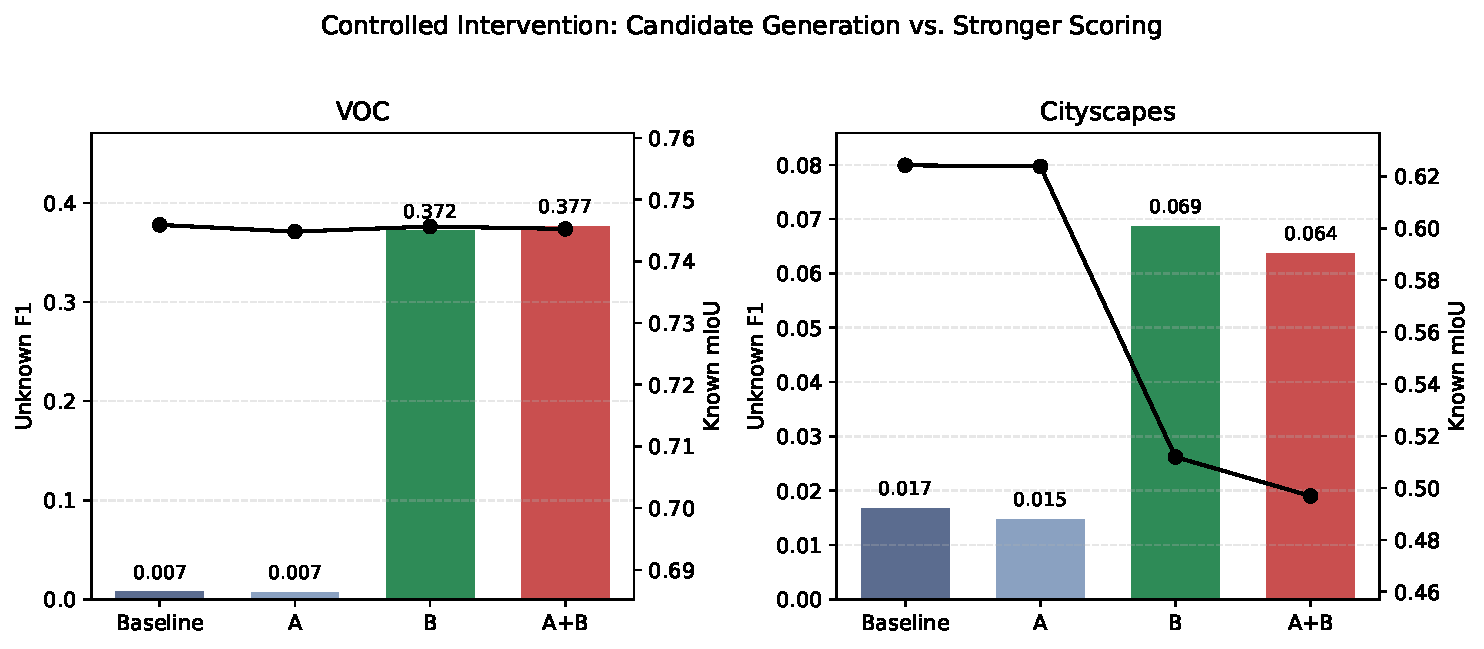
\includegraphics[width=\linewidth]{fig/intervention_bar.pdf}
  \caption{Controlled intervention results on VOC and Cityscapes. Bars show Unknown F1 and the overlaid line shows Known mIoU. The figure makes clear that stronger candidates (B) drive the dominant gain, while stronger scoring alone (A) is ineffective and can even hurt performance.}
  \label{fig:intervention}
\end{figure}

\subsection{Candidate Filter Ablation}
\label{sec:exp:filter}

\begin{table}[!htbp]
  \caption{Best filter settings found for each dataset.}
  \label{tab:filter}
  \centering
  \begin{tabular}{llll}
    \toprule
    Dataset & $\tau_{\text{area}}$ / $\tau_{\text{overlap}}$ / $\tau_{\text{fusion}}$ & Known mIoU & Unknown F1 \\
    \midrule
    VOC & 128 / 0.50 / 0.50 & 0.7457 & 0.3721 \\
    Cityscapes & 64 / 0.80 / 0.10 & 0.5833 & 0.0736 \\
    \bottomrule
  \end{tabular}
\end{table}

Table~\ref{tab:filter} summarizes the best validation settings, but the more important finding is the difference in sensitivity across datasets. On VOC, threshold choice has almost no effect. Across the scanned area and overlap ranges, Unknown F1 stays tightly clustered around 0.372 and Known mIoU remains essentially unchanged. This indicates that VOC already provides sufficiently clean complement candidates and that filtering only performs mild cleanup.

Cityscapes behaves very differently. Here, threshold choice materially changes the operating point. Stricter overlap tolerance increases recall but also admits substantial known leakage, while more conservative settings recover known performance at the cost of collapsing unknown gains. The best balanced setting, $\tau_{\text{area}}=64$, $\tau_{\text{overlap}}=0.8$, and $\tau_{\text{fusion}}=0.1$, reaches Known mIoU 0.5833 and Unknown F1 0.0736. By contrast, the more permissive configuration associated with the raw B intervention leaves Known mIoU near 0.512 with no meaningful extra unknown gain.

This ablation matters for the paper's interpretation. It shows that the Cityscapes trade-off is not simply a bad hyperparameter choice. Filtering can partially mitigate the leakage problem, but it cannot eliminate it. The dense-scene failure mode is therefore structural: when concept grounding does not fully cover important known classes such as vegetation, pole, or fence, the complement region remains too contaminated for score fusion to cleanly separate known leakage from true unknown content.

\subsection{Prompt-Form Ablation}
\label{sec:exp:prompt}

\begin{table*}[!t]
  \caption{Prompt-form ablation. UMR denotes unknown-mask recall on the prompt-form diagnostic subset.}
  \label{tab:prompt}
  \centering
  \begin{tabular}{llllll}
    \toprule
    Form & VOC UMR@0.5 & VOC F1 & Cityscapes UMR@0.1 & Cityscapes F1 & Interpretation \\
    \midrule
    Direct negation & 0.0000 & 0.0075 & 0.0000 & 0.0167 & No usable response \\
    Generic concept & 0.0000 & 0.0368 & 0.0000 & 0.0445 & Weak, non-specific response \\
    Enumeration-then-complement & 0.5266 & 0.3721 & 0.1220 & 0.0736 & Only consistently usable form \\
    Negative exemplar & 0.0000 & 0.0700 & 0.0000 & 0.0235 & Unstable and weak \\
    \bottomrule
  \end{tabular}
\end{table*}

The prompt-form ablation directly answers a likely reviewer question: is the method merely one prompt-engineering choice among many? Table~\ref{tab:prompt} suggests the answer is no. Direct negation fails completely on both datasets, with zero UMR and no usable masks. Generic concept prompts sometimes produce outputs, but those outputs are too unspecific to anchor reliable unknown candidates. Negative exemplars also fail to produce stable gains despite additional engineering effort.

Enumeration-then-complement is the only prompt form that consistently produces meaningful candidates. On VOC it reaches UMR@0.5 of 0.5266 and supports the full-system Unknown F1 of 0.3721. On Cityscapes the prompt-level candidate quality is weaker, but it is still the only form that yields a non-trivial structural signal, reaching UMR@0.1 of 0.1220 and F1 of 0.0736. This is an important methodological point: the adopted design is not arbitrary, but forced by the capability boundary of the current concept-promptable interface.

\subsection{Backbone Comparison: Native \samthree{} vs. \samtwo{}+\clip{}}
\label{sec:exp:backbone}

\begin{table}[!htbp]
  \caption{Backbone comparison under the full-system A2 setting.}
  \label{tab:backbone}
  \centering
  \begin{tabular}{lll}
    \toprule
    Backbone & VOC mIoU / F1 & Cityscapes mIoU / F1 \\
    \midrule
    Baseline SASeg & 0.7459 / 0.0075 & 0.6242 / 0.0167 \\
    \samthree{} PCS + L2 & 0.7457 / 0.3719 & 0.5833 / 0.0736 \\
    \samtwo{}+\clip{} + L2 & 0.7393 / 0.2224 & 0.6222 / 0.0330 \\
    \bottomrule
  \end{tabular}
\end{table}

The backbone comparison tests whether the paper's main effect is specific to native \samthree{} Promptable Concept Segmentation or instead depends on a more general capability combination. The answer is mixed but informative. On VOC, the orchestrated \samtwo{}+\clip{} alternative reproduces a substantial part of the effect, raising Unknown F1 from 0.0075 to 0.2224 while keeping Known mIoU relatively stable at 0.7393. This confirms that the mechanism is not exclusive to a single proprietary interface.

At the same time, native \samthree{} remains clearly stronger. On VOC, \samthree{} reaches 0.3719 Unknown F1, outperforming \samtwo{}+\clip{} by about 0.15 absolute. On Cityscapes, the gap is also substantial: \samthree{} reaches 0.0736 Unknown F1 under the best filter, whereas \samtwo{}+\clip{} only reaches 0.0330 while providing almost no meaningful L1-to-L2 separation. The simplest interpretation is that the method depends on the joint availability of class-agnostic mask generation and reliable concept grounding, and that native \samthree{} currently supplies that combination more effectively than the orchestrated alternative.

\begin{figure}[!htbp]
  \centering
  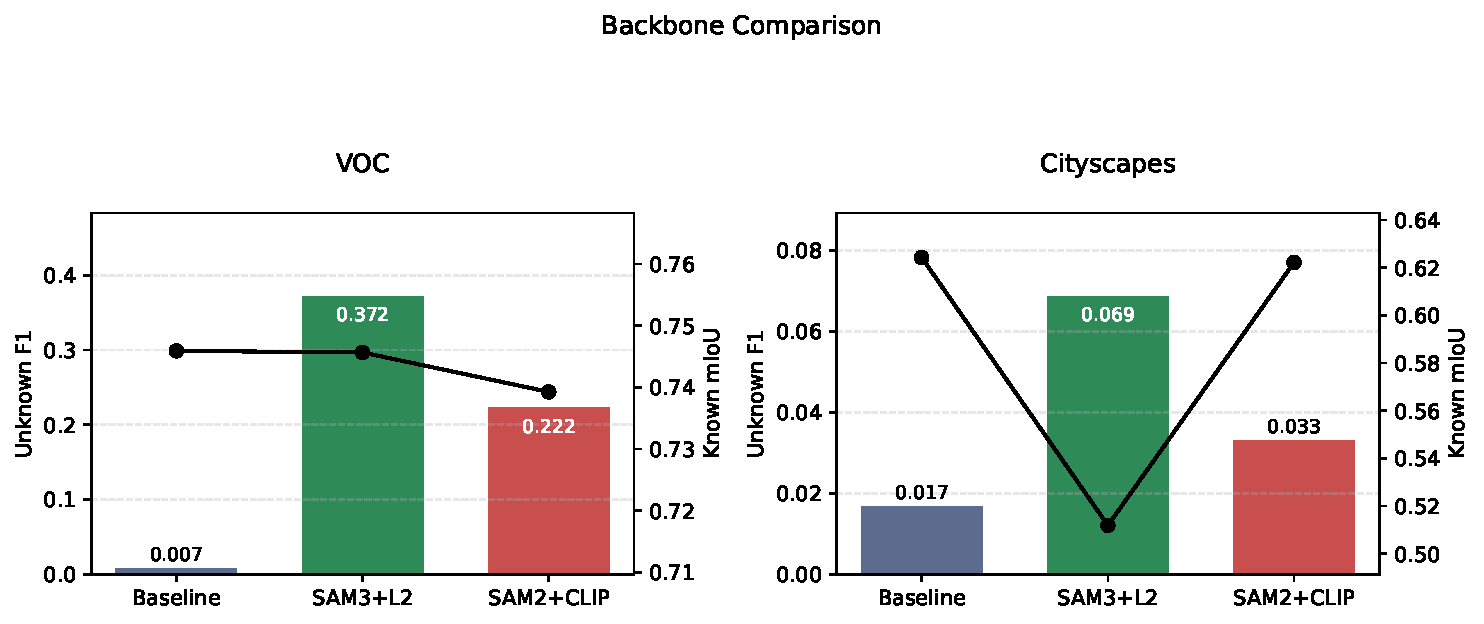
\includegraphics[width=\linewidth]{fig/backbone_comparison.pdf}
  \caption{Backbone comparison under the full-system A2 setting. Bars show Unknown F1 and the overlaid line shows Known mIoU. The orchestrated \samtwo{}+\clip{} alternative partially reproduces the effect, but native \samthree{} remains substantially stronger.}
  \label{fig:backbone}
\end{figure}

\subsection{SMIYC Official Evaluation}
\label{sec:exp:smiyc}

The SMIYC section is included for cross-benchmark mechanism validation, not for leaderboard competition. We report our own baseline alongside L1 and L2 under the official public-validation evaluator and explicitly state that hidden-test leaderboard systems are trained for a different objective with stronger task-specific supervision.

\begin{table*}[!t]
  \caption{SMIYC official public-validation results.}
  \label{tab:smiyc}
  \centering
  \begin{tabular}{llllllll}
    \toprule
    Dataset & Variant & Pix AP & Pix Best F1 & SegEval F1 mean & F1@25 & F1@50 & F1@75 \\
    \midrule
    RA21 & Baseline & 0.5937 & 0.5186 & 0.0326 & 0.0732 & 0.0240 & 0.0114 \\
    RA21 & L1 & 0.3436 & 0.5146 & 0.2990 & 0.4000 & 0.3111 & 0.1778 \\
    RA21 & L2 & 0.6211 & 0.5459 & 0.0313 & 0.1007 & 0.0278 & 0.0000 \\
    RO21 & Baseline & 0.4989 & 0.5117 & 0.0766 & 0.1600 & 0.0690 & 0.0139 \\
    RO21 & L1 & 0.1363 & 0.2197 & 0.2039 & 0.2333 & 0.2140 & 0.1429 \\
    RO21 & L2 & 0.5330 & 0.5256 & 0.0740 & 0.1695 & 0.0824 & 0.0235 \\
    \bottomrule
  \end{tabular}
\end{table*}

An important observation in this section is that L2 improves pixel-level metrics while L1 can remain stronger on instance-level SegEval metrics. This exposes a structural limitation of mean-score mask filtering: it improves purity at the cost of instance completeness when score distribution is spatially non-uniform within a large anomaly region.

Under the official pixel-level evaluator, L2 behaves as expected. On RoadAnomaly21, AP rises from 0.5937 to 0.6211 and Best F1 from 0.5186 to 0.5459. On RoadObstacle21, AP rises from 0.4989 to 0.5330 and Best F1 from 0.5117 to 0.5256. These gains are directionally consistent with the unified-protocol results and support the claim that the complement mechanism transfers beyond the paper's native evaluation setup.

However, the instance-level SegEval metrics reveal a different pattern. On both road datasets, L1 substantially outperforms L2 in F1 mean: 0.2990 vs.\ 0.0313 on RoadAnomaly21, and 0.2039 vs.\ 0.0740 on RoadObstacle21. This is not a contradiction, but a clue. Mean-score mask filtering improves pixel purity by dropping low-confidence regions, yet it can also fragment or discard large anomaly instances whose scores are spatially non-uniform. The resulting outputs score better on pixel-wise purity while becoming worse at preserving whole anomaly instances.

We report this mismatch explicitly because it sharpens the paper's scope. The proposed method is effective at generating and purifying unknown candidates, but the current L2 aggregation is not instance-preserving. This limitation is especially visible under the SMIYC official evaluator and motivates future work on score aggregation schemes that preserve instance completeness rather than relying on a single per-mask mean.

\subsection{Medical CT as a Failure Boundary}
\label{sec:exp:medical}

The medical experiments are reported as a deliberate boundary analysis. The key message is not that the proposed mechanism is universally effective, but that it depends on the foundation model's ability to ground known concepts in the target domain. On CT data, that prerequisite collapses, so the complement mechanism never receives a meaningful known-union estimate in the first place.

The initial feasibility probe on Synapse already shows the problem. Among the tested known-organ prompts, only \textit{liver} produces strong grounding (mean best IoU 0.810), and \textit{stomach} yields a weak partial response (0.265). Prompts for kidney, spleen, pancreas, and aorta are effectively unusable, while pathology-style prompts such as \textit{tumor}, \textit{lesion}, or negation-style complement prompts fail entirely. This means the method never starts from a reliable known explanation of the scene.

The stage-0.5 $\beta$ probe confirms that the downstream complement signal remains unusable even when the rough known union is not totally collapsed. On Synapse, the known-union IoU against known anatomy reaches 0.6517, and the complement region attains very high unknown recall (0.9358), but its precision is only 0.0454, with known leakage 0.9546. In other words, almost everything left in the complement is still known anatomy rather than a meaningful unknown candidate. This behavior is qualitatively different from VOC and even from Cityscapes, where the complement retains at least some task-relevant signal.

We therefore present medical CT as a failure boundary of the current foundation model rather than as a failure of the complement principle itself. The evidence suggests that the mechanism depends first on concept grounding coverage, and only second on downstream filtering. When the model cannot ground the known domain concepts in the first place, complement prompting has no reliable substrate on which to operate.

\begin{figure*}[!t]
  \centering
  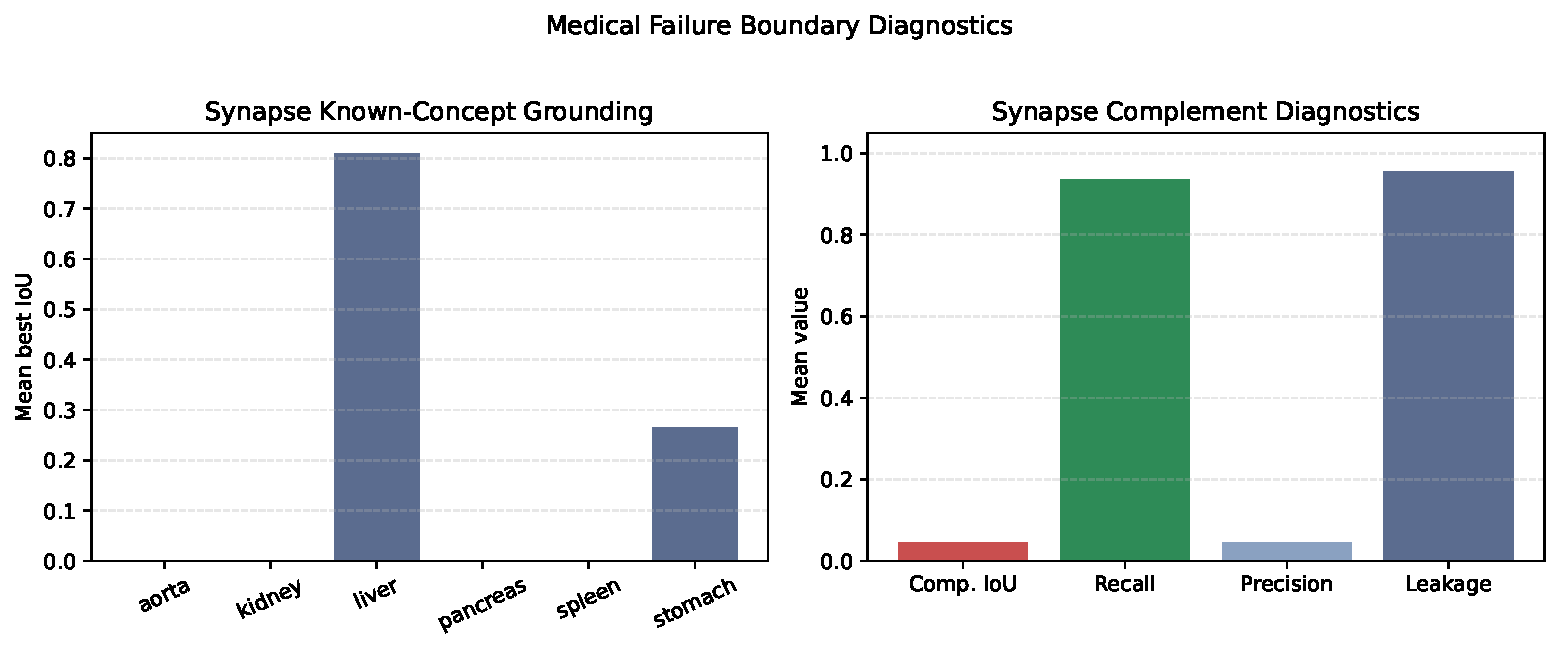
\includegraphics[width=0.92\textwidth]{fig/medical_diagnostics.pdf}
  \caption{Medical failure diagnostics on Synapse. Left: mean best IoU for known-organ concept grounding, showing that only a small subset of anatomy is grounded reliably. Right: complement diagnostics from the stage-0.5 probe, where recall remains high but precision collapses and known leakage dominates, preventing useful unknown candidate generation.}
  \label{fig:medical-failure}
\end{figure*}

\subsection{Candidate Quality Diagnostics}
\label{sec:exp:diagnostics}

The candidate diagnostics provide a compact explanation for why the method succeeds in some regimes and fails in others. On the VOC diagnostic subset, the complement signal is already strong before score fusion: known-union IoU against known content is 0.6956, complement IoU against unknown content is 0.8885, unknown recall in the complement reaches 0.9997, and precision remains high at 0.8887. This is exactly the regime in which score fusion only needs to perform light cleanup, which explains the near-zero known-side degradation in the final full-system result.

Cityscapes occupies an intermediate regime. The diagnostic known-union IoU is only 0.5324, complement IoU against unknown is 0.1709, unknown recall is still very high at 0.9898, but precision falls to 0.1711 and known leakage rises to 0.8289. In other words, the complement still finds most unknown content, but it also contains a large amount of known residue. This explains both why L1 is unusable and why L2 helps but cannot fully resolve the trade-off.

Medical CT is the failure regime. There, the issue is no longer just leakage, but representational collapse: the foundation model does not ground most known anatomy reliably, so the complement is not even anchored to a correct foreground decomposition. Read together, these diagnostics support the paper's regime-based interpretation: the method succeeds when concept grounding coverage is high and scene density is moderate, trades off when grounding is partial in dense scenes, and fails when grounding collapses in an out-of-domain modality.

\section{Discussion}
\label{sec:discussion}

\subsection{The Real Dependency Is a Capability Combination}
\label{sec:discussion:capability}

The backbone substitution results suggest that the proposed method should not be interpreted as ``a new way to use \samthree{}'' and nothing more. The deeper dependency is the combination of two capabilities: class-agnostic mask generation and concept-level grounding. The first capability is needed to decompose a residual foreground region into coherent mask candidates. The second is needed to explain away the known part of the scene so that the residual complement carries meaningful unknown structure. Either capability in isolation is insufficient.

\samthree{} is currently the most natural provider of this combination, which explains why the main method is strongest with native Promptable Concept Segmentation. But the partial success of the \samtwo{}+\clip{} orchestration shows that the broader claim is not model-specific. Once these two capabilities are available in the same pipeline, zero-shot unknown candidate generation becomes possible. What changes from model to model is how cleanly and how robustly the two capabilities are realized.

This capability-level reading matters for the paper's long-term relevance. Absolute numbers may change as foundation models improve, but the structural lesson should remain: open-world dense segmentation can benefit from concept-promptable foundation models not because they magically solve unknown understanding, but because they can supply the missing candidate structure that conventional anomaly scoring lacks.

\subsection{Transferable Findings Beyond \samthree{}}
\label{sec:discussion:transfer}

Several findings of the paper are intended to outlive the specific model instance used here. First, direct negation is not currently a reliable route to structured unknown discovery in concept-promptable segmentation. The successful mechanism is not ``ask for what is unknown,'' but ``explain what is known, then use the residual.'' Second, high-recall complement candidates are useful only if they are followed by some form of region-level purification. The contrast between L1 and L2, and the SMIYC pixel-versus-instance divergence, both point to this conclusion.

Third, pixel-level ranking should be treated as a necessary but insufficient condition for structured abstention. This is arguably the most transferable finding in the paper. The intervention results show that high AUROC does not answer the operational question that matters in dense prediction: can the system produce a usable unknown region? Fourth, the real A2 bottleneck is candidate generation rather than score strengthening. The fact that stronger scoring alone fails across datasets while stronger candidates drive the main gains is unlikely to be specific to one model release.

Finally, the paper suggests a more general template for future work. If stronger concept-promptable models become available, especially domain-adapted ones, they can be inserted into the same pipeline and evaluated through the same reasoning lens: how well do they explain known content, how clean is the complement, and what kind of region-level purification is needed afterward. In this sense, the paper contributes not only one method, but also a way of thinking about foundation-model assistance in open-world dense segmentation.

\subsection{Limitations}
\label{sec:discussion:limitations}

The first limitation is evaluative. Much of the paper's core analysis is organized around the SASeg A1/A2 framing. We believe this framing is useful precisely because it separates ranking quality from structured output quality, but it is not yet a community standard. For that reason, the cross-benchmark SMIYC results are important, yet they do not fully substitute for the protocol-specific claims made in the main experiments.

The second limitation is that the dense-scene trade-off is not solved. Cityscapes demonstrates that the proposed mechanism can improve unseen-unknown structuring in crowded natural scenes, but only by accepting a non-trivial degradation in known-class segmentation. Threshold tuning mitigates this effect, but it does not eliminate it. The current method therefore works best in regimes where the known explanation is already reasonably complete and the residual complement has a workable signal-to-noise ratio.

The third limitation is domain coverage. On medical CT, the method fails not because complement prompting is conceptually wrong, but because the underlying foundation model lacks sufficient grounding coverage for the modality. This sharply limits the present paper's direct applicability to domains far from the training distribution of the concept-promptable model. Domain-adapted concept grounding remains an external dependency rather than something solved here.

The fourth limitation is structural quality at the instance level. Mean-score mask filtering is a blunt aggregation strategy. It is effective at improving pixel-level purity, but the SMIYC SegEval results show that it can fragment or suppress whole anomaly instances. A better instance-preserving aggregation rule is an obvious next step and may materially change the balance between L1-style completeness and L2-style purification.

The fifth limitation is temporal. The paper uses a particular \samthree{} release and a particular orchestration baseline. Future foundation-model updates may change absolute performance and perhaps even alter some prompt-interface behaviors. For this reason, we deliberately frame our strongest claims at the capability level rather than tying them too tightly to one release version.

\section{Conclusion}
\label{sec:conclusion}

This paper addresses the specific open problem left by SASeg: how to generate unknown candidates for A2 unseen-unknown structuring without introducing unknown supervision or retraining the segmentation model. We show that concept-promptable foundation models make a simple inference-time solution possible. By enumerating known classes, taking their foreground complement, and filtering the resulting candidates with the frozen SASeg anomaly signal, \method{} turns a previously diagnostic bottleneck into a tractable mechanism.

The main contribution of the paper is not only the resulting performance gain, although that gain is substantial on the right datasets. More importantly, the paper turns a correlational diagnosis into intervention-style empirical evidence. Stronger scoring alone does not resolve A2. Stronger candidates do. This establishes candidate generation, rather than anomaly-score quality, as the dominant structural bottleneck in the setting studied here.

At the same time, the paper does not claim universal success. Across six datasets, the experiments identify a clear regime structure. Object-isolated natural-image settings such as VOC form the effective regime. Dense urban scenes such as Cityscapes form a partial regime with a real known--unknown trade-off. Medical CT constitutes a failure regime under the current foundation model because concept grounding collapses outside the model's visual domain. The SMIYC results further show that pixel-level purification and instance-level completeness remain in tension under simple mean-score filtering.

Taken together, these results suggest a broader outlook for open-world dense segmentation. Concept-promptable foundation models can serve as zero-shot candidate generators when they provide adequate concept grounding and class-agnostic decomposition, but they do not remove the need for careful region-level selection and boundary analysis. Future progress will likely come from stronger domain coverage and better instance-preserving score aggregation rather than from score sharpening alone. In that sense, this paper closes one open problem while also clarifying the next ones.

\appendix

\section{Supplementary Material}
\label{sec:appendix}

The supplementary material includes additional visualizations for fusion-threshold sensitivity, prompt-form ablation, and the SMIYC pixel-level versus instance-level trade-off. Other potential supplementary items include per-class analyses, complete prompt templates, additional qualitative examples, and implementation details for the \samtwo{}+\clip{} orchestration path.

% TODO: Replace placeholder bibliography entries with the actual paper bib file.
\bibliographystyle{cas-model2-names}
\bibliography{cas-refs}

\end{document}
